\section{Prototypes in sprint 2}
To facilitate some of the feedback received during sprint 1 and visualize some of the user stories to be implemented in sprint 2 and beyond we revised the prototypes.
One of the previous prototypes was changed and another was added.

\subsubsection{The prototype for changing to guardian mode}
When changing to guardian mode the system should prompt the user for a password.
This was implemented as a completely new screen in the previous prototypes.
This was deemed to be unnecessary and too complicated.
As such, it was changed to be a notification popup rather than a new screen in this sprint.
The two prototypes can be seen in \autoref{fig:revised_guardian_switch}.

\begin{figure}[H]
    \begin{subfigure}{0.5\textwidth}
    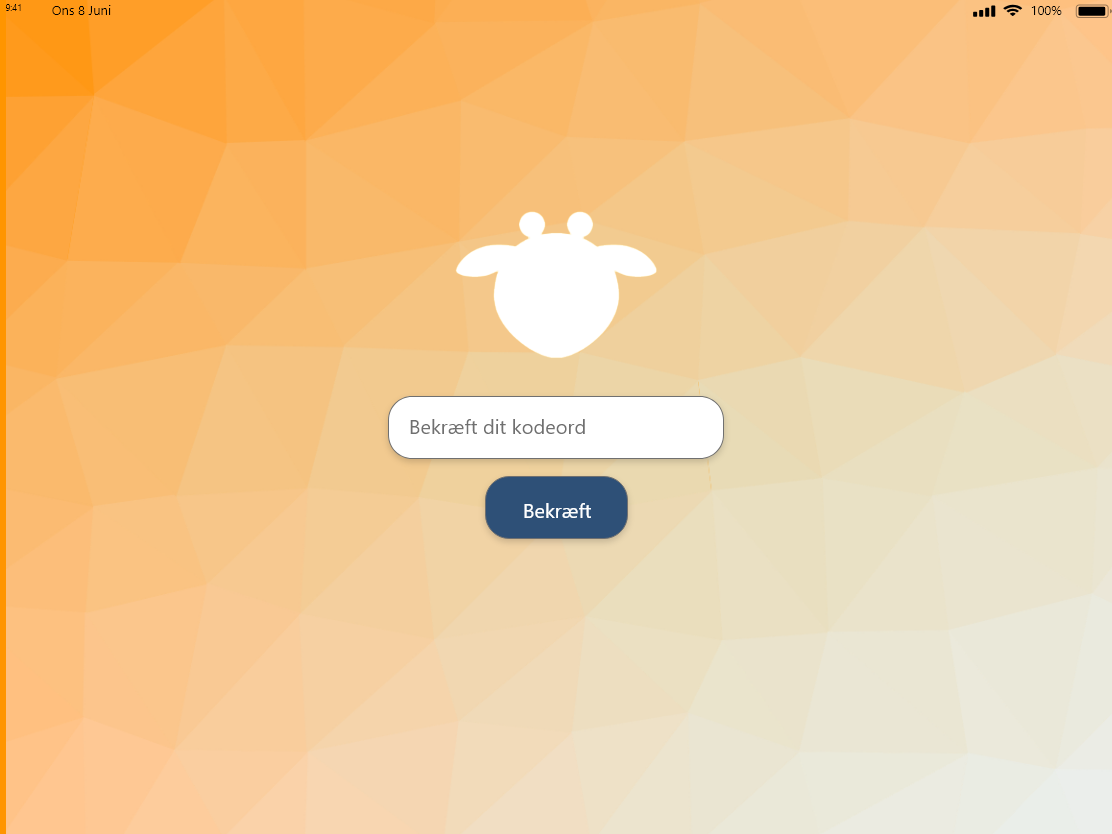
\includegraphics[width=1\linewidth, height=5cm]{guardian_switch_confirm.png} 
    \caption{The previous guardian screen}
    \label{fig:previous_guardian_screen}
    \end{subfigure}
    \begin{subfigure}{0.5\textwidth}
        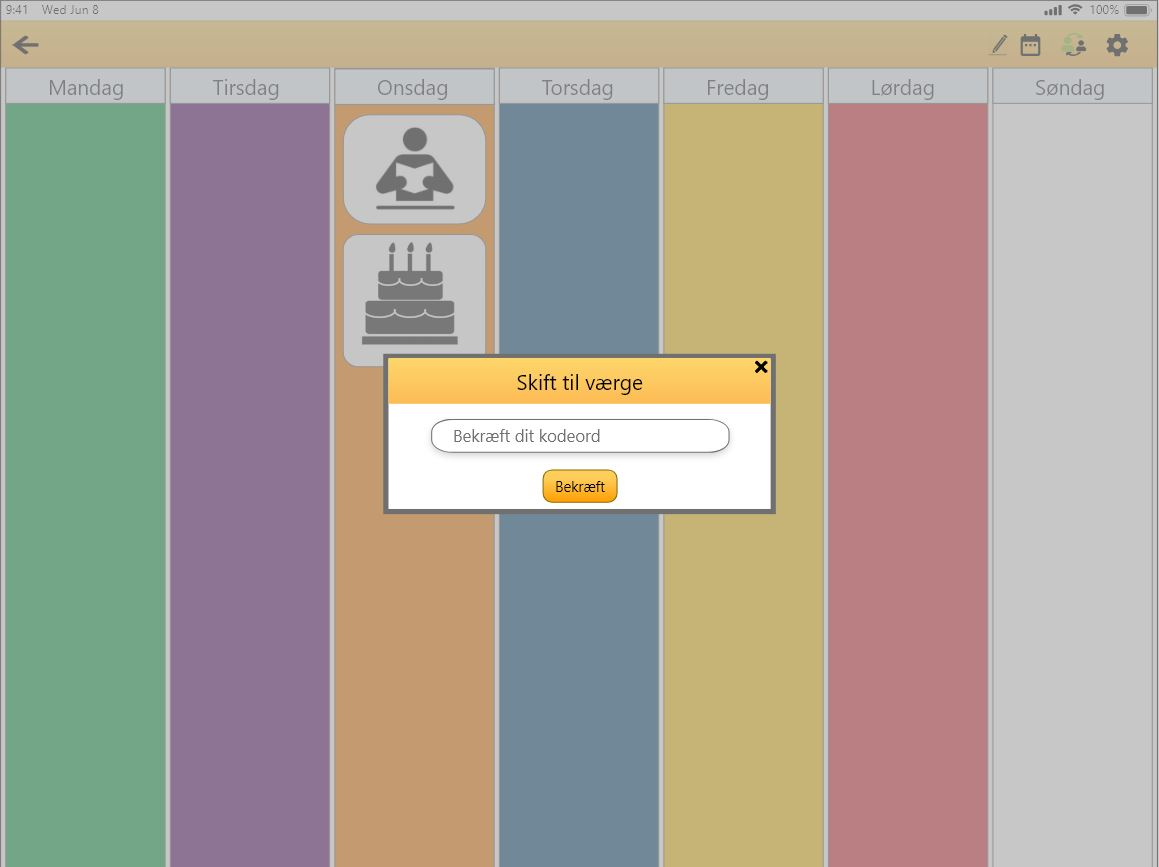
\includegraphics[width=1\linewidth, height=5cm]{new_guardian_popup.JPG}
    \caption{The proposed new guardian popup}
    \label{fig:new_guardian_popup}
    \end{subfigure} 
    \caption{This figure shows the old screen for switching to guardian mode and the new popup solution.}
    \label{fig:revised_guardian_switch}
\end{figure}

\subsubsection{Citizen selection}
As discussed in \autoref{interview13-3}, an additional layer when selecting citizens would be preferable.
To facilitate this we constructed a new prototype based on the design of choosing a citizen as shown in \autoref{prototype-comp}.
Rather than show pictures of the students, it would instead show folders representing each class.
Opening a folder leads to the pictures of the students in the class, such that one can be selected.
This prototype can be seen in \autoref{fig:class_folder_prototype}.

\begin{figure}[h]
    \centering
    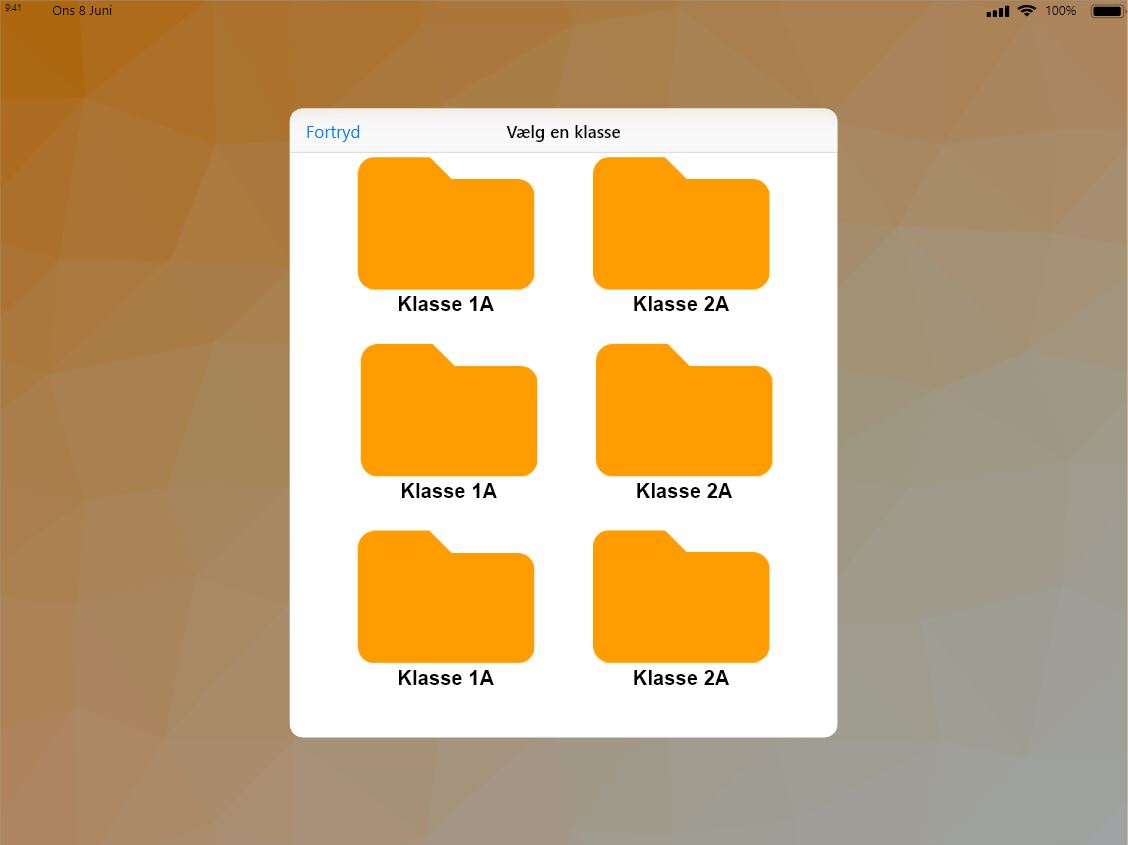
\includegraphics[width=0.6\textwidth]{class_folder.JPG}
    \caption{The new prototype for selecting a class before a citizen.}
    \label{fig:class_folder_prototype}
  \end{figure}
